\chapter{Theory}

This chapter describes the underlying concepts which are used throughout the thesis. 

\section{Vector Tiles}\label{part1_vector_tiles}

Instead of delivering a image of the map to a client like a browser or mobile phone, only the vector representation of the data is sent to the client which is using less data and allows more interactive, dynamic  and resolution independent cartography. This is only possible since clients have more powerful hardware and are able to render maps themselves.

\begin{figure}[H]
\centering
\includegraphics[width=1.0\textwidth]{images/vector_raster_example}
\caption{Vector and client representation of a map section}
\end{figure}

Google introduced the XYZ tiling scheme \cite{v_1_wiki.openstreetmap.org_2015} back in 2005 because it is not scalable to deliver an image of the map tailored to the viewport of the client.
The idea is to divide the map image into a grid where clients request idempotent raster images by using tile indizes instead of coordinates. This allows caching on the browser and server side and results in a smoother map experience.
The same approach can be applied to vector data. Instead of delivering the vector data for the entire viewport the vector data is sliced into tiles. \\\\

\begin{figure}[H]
\centering
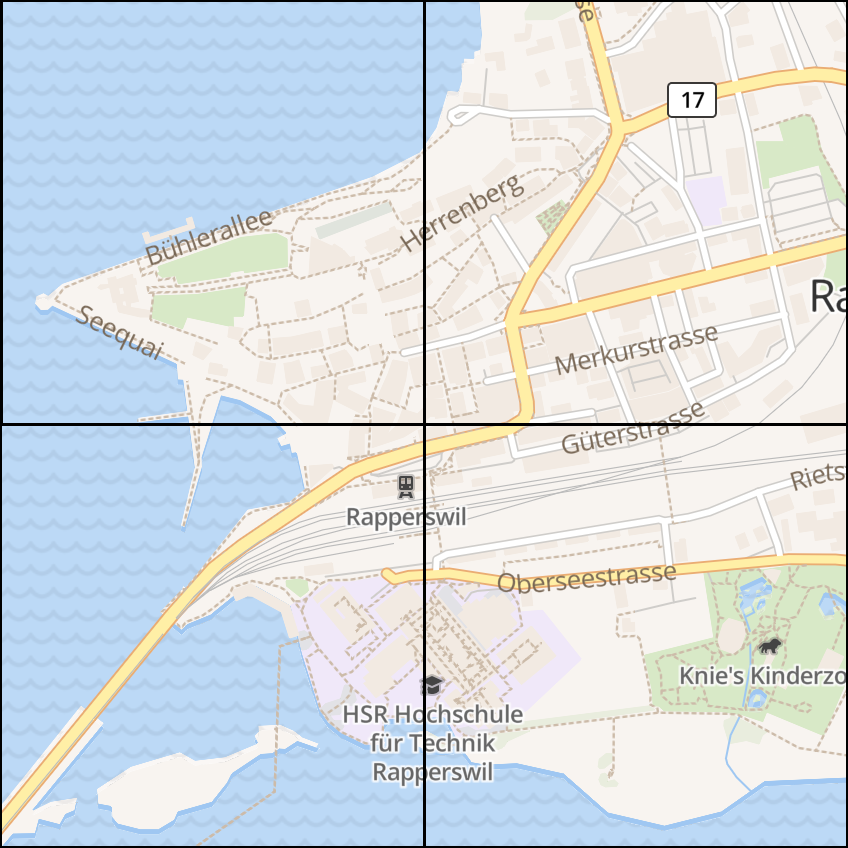
\includegraphics[width=0.5\textwidth]{images/tiled_raster}
\caption{Tiled raster map}
\end{figure}

Vector tiles contain all the geometry and metadata needed for a specific tile. This makes them more flexible than serving raster tiles, because a different style can be applied on the fly. For example based on the language preference of the browser language-specific city labels can be shown.\\

The data inside of vector tiles is structured into layers and features. A vector tile can have multiple layers such as roads, landuse or water (elaborated in \autoref{database-schema}). Each layer consist of one or multiple features. A feature contains a geometry field (either of type point, linestring or polygon) and metadata such as label translations.

\subsection*{Mapbox Vector Tile Specification}\label{part1_vector_tile_specification}

The Mapbox Vector Tile Specification defines how to encode tiled vector data using Protobuf. More details about the encoding and internal structure of vector tiles can be found in the specification\cite{104_mapbox.com_2016}.

\section{XYZ Coordinate Schema}\label{part1_xyz_coordinates}

For tiling the vector tiles the XYZ numbering schema has been used.
The tiles are organized in a 3-dimensional coordinate system (\texttt{x/y/z}) where \texttt{x} and \texttt{y} represent the axes and \texttt{z} the zoom level. As users zoom into a map each tile is replaced by four children within the tile.

\begin{figure}[H]
\centering
\includegraphics[width=0.5\textwidth]{images/xyz_scheme}
\caption{XYZ coordinate schema}
\end{figure}

\section{OpenStreetMap Data Model}\label{openstreetmap_data_model}

The data model of \osm{} consists of objects of type node, way and relation. Nodes define points in space, ways define linear features and relations define how objects relate to each other\cite{1_osm_wiki_2016}.

\begin{figure}[H]
\centering
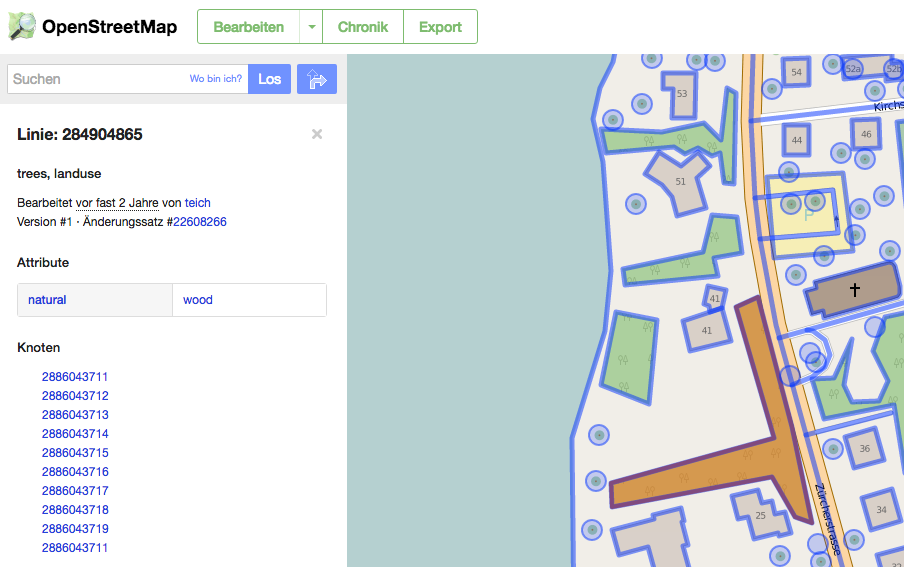
\includegraphics[width=0.8\textwidth]{images/osm_data_model}
\caption{Example of object tagged with natural=wood}
\end{figure}

Every object can have one or more tags associated with it. Tags define the meaning of a certain object. A tag consists of a key/value pair for example the tag \textbf{natural=wood} is used to define areas which are covered in trees. OSM tags are not strictly defined and users can add their own tags but there are many conventions which should be followed.